\section{Background Estimation}
\label{sec:background}

%Backgrounds: The backgrounds should be evaluated and this should include CR/VR plots with the full data (full run-2 analyses) or at least a representative majority of the data (analyses during data-taking); 
%exceptionally a minor background could be still under finalization, but in this case a short timescale should be envisaged for its completion, or it should be a background that does not affect the accuracy of the result. ( a 10% background on a 10% accuracy measurement is not a minor background)

The transverse mass \mt~is chosen as the search variable due to the potential for the SVJ signal to create a resonant shape around the mass of the $Z'$. \mt~is the total transverse mass of the two leading jets and the \met~, expressed in Equation~\ref{eq:mt} as:

\begin{equation}
m_T^2 = [E_{T,jj} + \met~]^2 - [\vec{p}_{T,jj} + \vec{p}_T^{\text{miss}}]^2
\label{eq:mt}
\end{equation}

where $E_{T,jj}$ is the transverse energy of the dijet system. We take $E_{T,jj} = m_{jj}^2 + |\vec{p}_{T,jj}|^2$, where $m_{jj}^2$ is the invariant mass of the two leading jets, and $\vec{p}_{T,jj}$ is the vector sum of the \pt~of the two leading jets. \mt~is selected as the search variable in place of simpler invariant mass $m_{jj}$ because substantial energy from the Z' decay is captured in the \met~. Therefore incorporating \met~into \mt~improves the resonance around the mass of the $Z'$. \par

Figure~\ref{fig:mt_mass} illustrates the resonance in \mt~of the SVJ signals.
\begin{figure}[!htbp]
\centering
    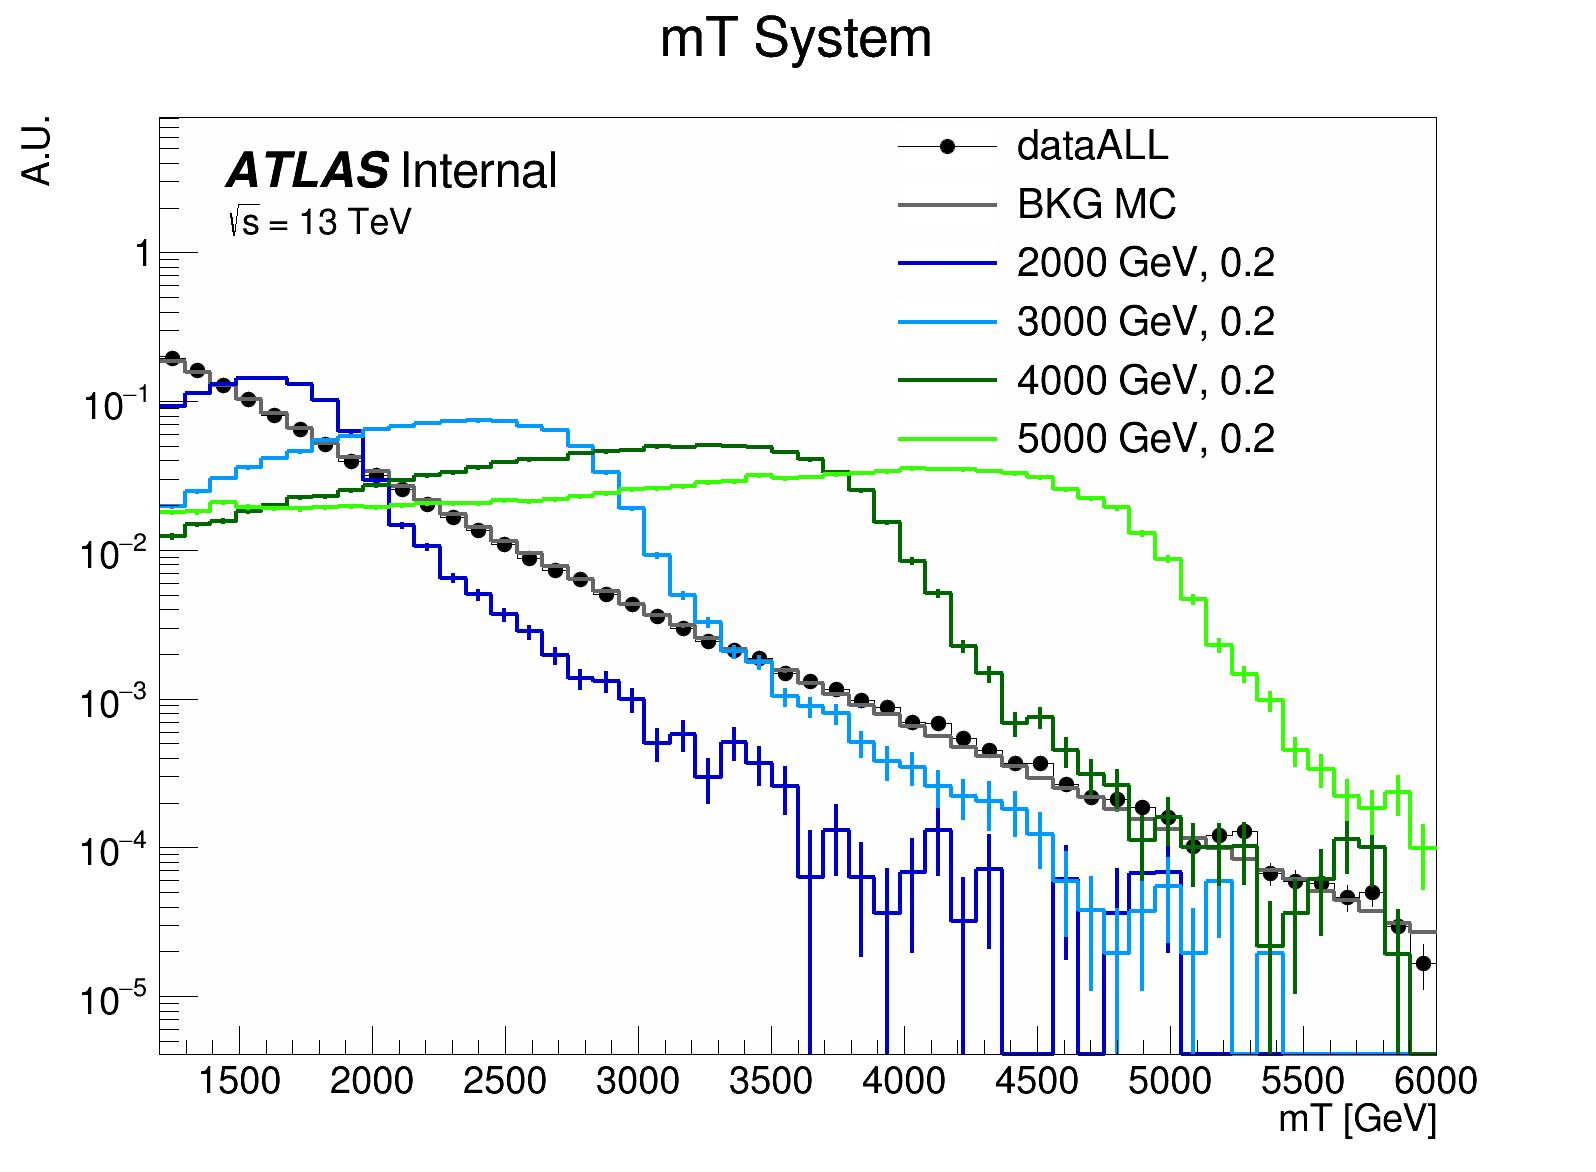
\includegraphics[width=0.49\textwidth]{figures/ch8/mt_mass_lowrinv}
    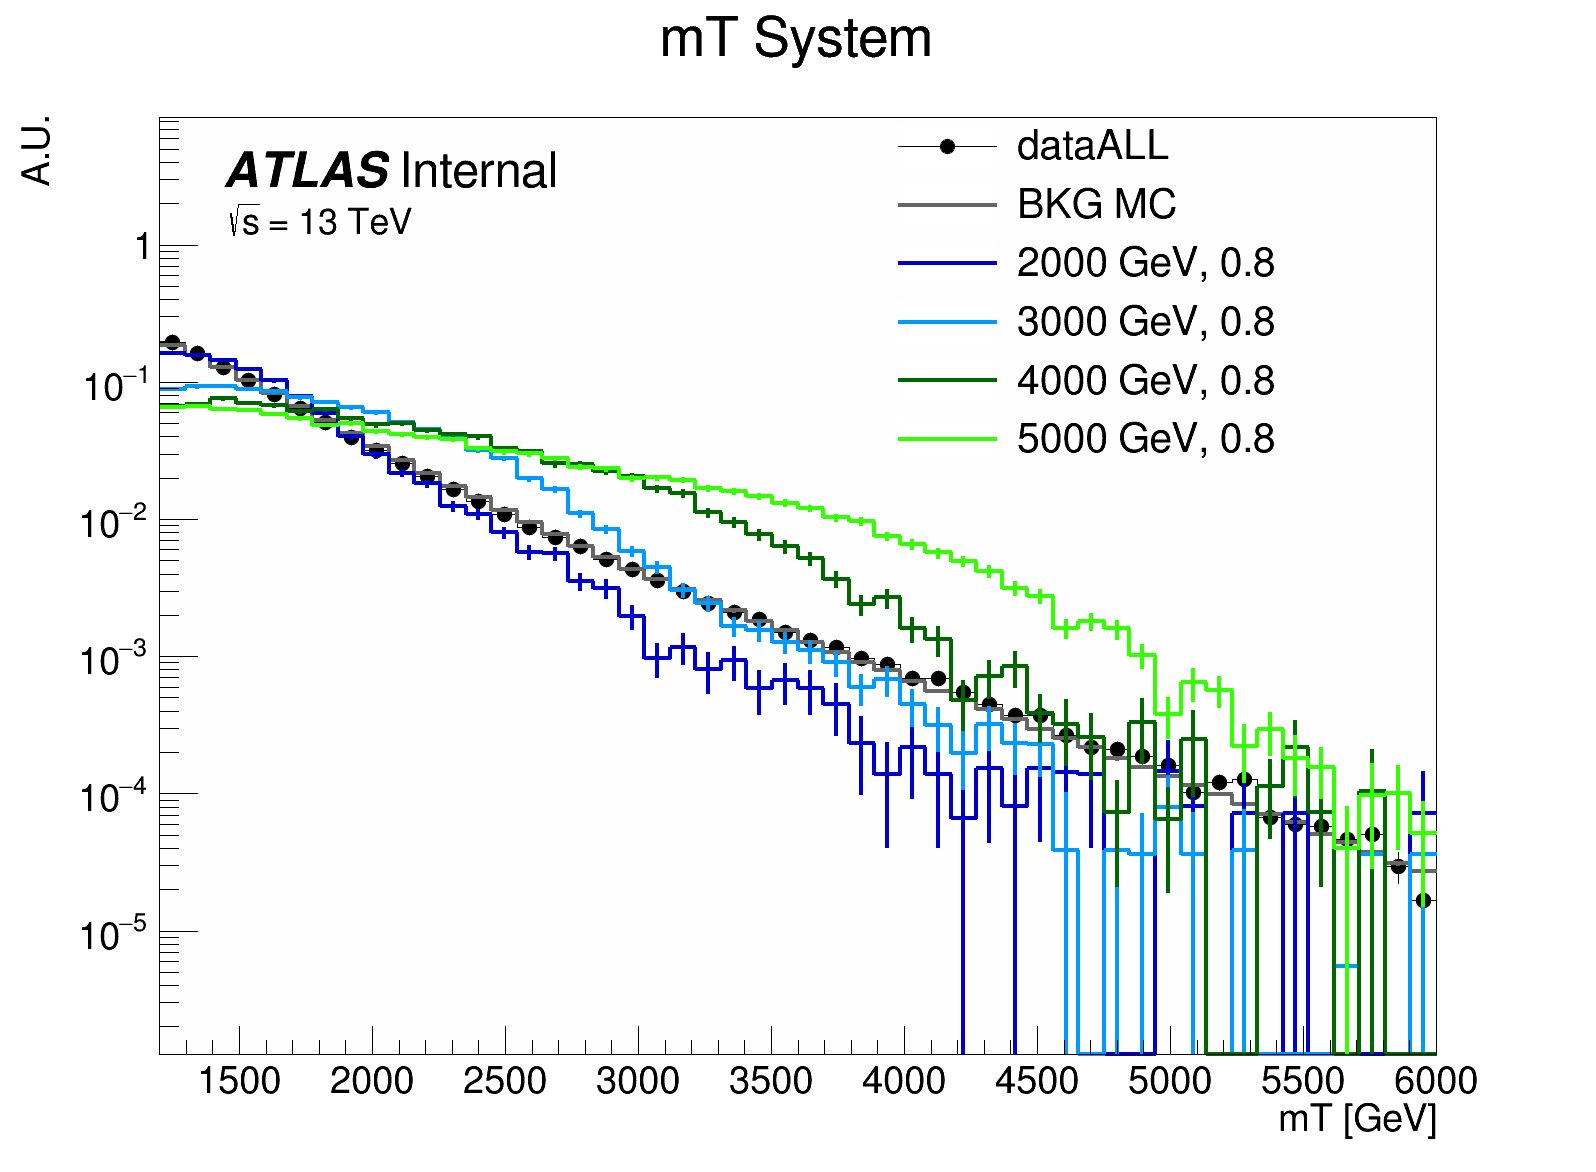
\includegraphics[width=0.49\textwidth]{figures/ch8/mt_mass_highrinv}
    \caption{The resonant shape of the SVJ signals in \mt~, in contrast to the smoothly falling \mt~background. The high \rinv~signals (right) boast a wider shape, making them more difficult to detect, while the low \rinv~signals(left) produce a more narrow resonance in \mt~. 
    \label{fig:mt_mass}}
\end{figure}

%This is done via a data template for the shape of \mt~taken from a CR that is orthogonal to the SR, but still close in SM process contribution and kinematic phase space. 
%A polynomial fit is then performed to describe the shape of \mt~in the SR.
%The polynomial is constructed using the CR data template, and validated to data in a VR that is similarly orthogonal to both the CR and SR.
The SM background in the SR is predominantly composed of QCD events, and due to the poor modeling of QCD at high energies by MC, it is estimated in a fully data-driven way. 
An empirical functional form is used for the background shape of \mt.
The ability of this function to model the background behavior is tested both the CR and the VR for each analysis strategy. The shape parameters are left free in all the fits.

The fits are performed for 1500 GeV $<$ \mt~ $<$ 6000 GeV.
The polynomial chosen is a standard 5-parameter function used in several similar dijet search analyses such as \cite{darkjets} \cite{smooth_bkg} \cite{cms_svj} and shown in Equation~\ref{eq:bkgpoly}:
\begin{equation}
f(x) = p_1(1-x)^{p_2}x^{p_3+p_4 lnx+p_5ln^2x}
\label{eq:bkgpoly}
\end{equation}
Here x = m$_{jj}$/$\sqrt{s}$ and the $p_i$ are free parameters.
The fit function is required to be fully positive, and the \mt~distribution is fit to 90 even-width bins.
The resulting fit shape is used as the background estimation for both the SVJ Fit strategy and the Discovery strategy. 
Validation of the fit and its ability to both model the background and detect signal are shown in Section~\ref{sec:fit_strategy}.
Higher order polynomials were also considered, but an F-test was performed and the five parameter function was determined to be adequate and optimal for capturing the shape of the background.






